%% -*- coding: utf-8 -*-
\documentclass[12pt,pagesize,paper=192mm:108mm]{scrbook} 
%1920x1080 1280x720
\areaset[current]{192mm}{108mm}
\usepackage{calc}
\usepackage[T2A]{fontenc}
\usepackage[utf8]{inputenc}
\usepackage[english,russian]{babel}
\usepackage{microtype}
\usepackage{misccorr}
\usepackage{cmap}
%\usepackage[unicode=true]{hyperref}
\usepackage{graphicx}
\usepackage{amssymb}
\usepackage{amsmath}
%\usepackage{srcltx}
\usepackage{textcomp}
\usepackage{xspace}
%научные символы и смайлики \smiley \frownie
\usepackage{wasysym}
\usepackage{ccicons}
\begin{document}
\begin{titlepage}
  \vspace*{-0.5em}
  \begin{center}    
    \hspace*{3em}
    \begin{minipage}[t]{3em}
      
\includegraphics[width=\textwidth]{../BINP-logo}
    \end{minipage}\hfill
    \begin{minipage}{0.23\linewidth}
    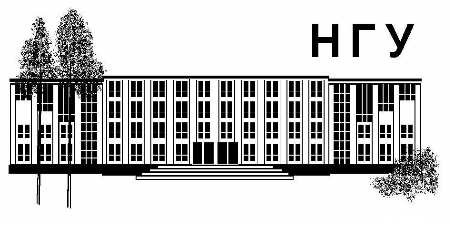
\includegraphics[width=\textwidth]{../NSU-logo}
    \end{minipage}
    \hfill
    \hspace*{6em}

    Кафедра теоретической физики физического факультета НГУ
    \medskip

    \Large
    Профессор Черняк В.\,Л.
    \bigskip

    \huge
    \textbf{Теория электрослабых взаимодействий}
    \bigskip

    \Large
    Лекция № 15
    \vfill

    % \normalsize
    % \begin{minipage}{0.65\linewidth}
    % \end{minipage}
    \vfill

\normalsize    Новосибирск 2013
  \smallskip

  \ccbysa
  \end{center}
\end{titlepage}
\newpage

\vspace*{-1em}
\begin{center}
 \vfill
  \begin{minipage}{0.66\linewidth}
    Оценки для нелептонных распадов в приближении факторизации на
    примере распадов:
    \begin{enumerate}
    \item $B^-\to D^0\pi^-$,
    \item $\bar{B}^0\to D^+\pi^-$,
    \item $\bar{B}^0\to D^0\pi^0$.
    \end{enumerate}

    Применение тождеств Фирца в эффективном лагранжиане с операторами
    \[O_1=\bar{d}\left(1-\gamma_5\right)\gamma^{\mu}u\bar{c}\left(1-\gamma_5\right)\gamma_{\mu}b\]
    и
    \[O_2=\bar{c}\left(1-\gamma_5\right)\gamma^{\mu}u\bar{d}\left(1-\gamma_5\right)\gamma^{\mu}b.\]
    Связь ширин нелептонных распадов в приближении факторизации
    с~формфакторами полулептонных распадов.  Зависимость полулептонных
    формфакторов от передачи импульса: полюсное приближение
    (резонансные вклады). Численные значения для формфакторов.
  \end{minipage}
  \vfill
  % Новосибирск 2013

  % \normalsize \ccbysa
\end{center}
\end{document}
